% Created 2025-04-29 Tue 19:32
% Intended LaTeX compiler: pdflatex
\documentclass[11pt]{article}
\usepackage[utf8]{inputenc}
\usepackage[T1]{fontenc}
\usepackage{graphicx}
\usepackage{longtable}
\usepackage{wrapfig}
\usepackage{rotating}
\usepackage[normalem]{ulem}
\usepackage{amsmath}
\usepackage{amssymb}
\usepackage{capt-of}
\usepackage{hyperref}
\usepackage{minted}
\usepackage{siunitx}
\author{Hankertrix}
\date{\today}
\title{Amino Acids \& Proteins Notes}
\hypersetup{
 pdfauthor={Hankertrix},
 pdftitle={Amino Acids \& Proteins Notes},
 pdfkeywords={},
 pdfsubject={},
 pdfcreator={Emacs 30.1 (Org mode 9.7.11)}, 
 pdflang={English}}
\begin{document}

\maketitle
\setcounter{tocdepth}{2}
\tableofcontents \clearpage\section{Definitions}
\label{sec:orgaed9b04}

\subsection{Proteinogenic}
\label{sec:orge7ae9d3}
Proteinogenic just means "protein creating", which means an amino acid that is proteinogenic is incorporated into proteins during translation.
\subsection{Physiological pH}
\label{sec:org3a5c7f9}
Physiological pH is about 7.35 - 7.45.
\subsection{Non-polar amino acids}
\label{sec:orgee4c63c}
Non-polar amino acids have side chains that are either aliphatic or aromatic. For example, proline has an aliphatic cyclic structure, whose amino group is a secondary amine.
\subsection{Polar amino acids}
\label{sec:org06d2433}
Polar amino acids have polar side chains that are neutral (uncharged) neutral pH.

A few examples:
\begin{itemize}
\item Serine (\textbf{Ser}) and threonine (\textbf{Thr}) has a hydroxyl (\(-OH\)) group, which are good nucleophiles that play a role in enzymatic activity.
\item Cysteine (\textbf{Cys}) has a thiol (\(-SH\)) group and two cysteine can oxidise to form a disulfide bond.
\item Glutamine (\textbf{Gln}) and Asparagine (\textbf{Asn}) have an amide group, which do not ionize at physiological pH.
\end{itemize}
\subsection{Acidic amino acids}
\label{sec:org0cc2453}
Acidic amino acids are amino acids that have acidic side chains, which are \textbf{negatively charged} at physiological pH. Glutamic acid (\textbf{Glu}) and aspartic acid (\textbf{Asp}) are the only acidic amino acids.
\subsection{Basic amino acids}
\label{sec:org5fd28b2}
Basic amino acids refer to amino acids that have basic side chains, which are \textbf{positively charged} at physiological pH. Histidine (\textbf{His}), lysine (\textbf{Lys}) and arginine (\textbf{Arg}) are the only basic amino acids. Histidine has an imidazole group, whose \(pK_a\) is \(\sim\) 6, which is very close to the physiological pH.
\subsection{Amphoteric}
\label{sec:org05b9e48}
An amphoteric substance is a substance that can react as either a base or an acid.
\subsection{Ampholyte}
\label{sec:orgb48882a}
Ampholyte refers to a molecule consisting of both positively and negatively charged components.
\subsection{Zwitterion (zwitterionic form)}
\label{sec:org6b4069b}
A zwitterion refers to a molecule or an ion having separate positively charged and negatively charged groups.
\subsection{Isoelectric point (pI)}
\label{sec:org5fad2f7}
The isoelectric point refers to the pH at which a molecule has zero net charge.
\[pI = \frac{pK_{a1} + pK_{a2}}{2}\]
\subsection{Proteins}
\label{sec:orgaef478d}
Proteins are \textbf{polymers} of amino acids, where the amino acids are joined \textbf{head-to-tail} by covalent peptide bonds.


The peptide backbone of a protein consists of the repeated sequence \(-H-C_{\alpha}-C_{\circ}\).

Where:
\begin{itemize}
\item "\(N\)" is the amide nitrogen of the amino acid
\item "\(C_{\alpha}\)" is the alpha carbon of the amino acid
\item "\(C_{\circ}\)" is the carbonyl carbon of the amino acid
\end{itemize}
\subsection{Peptide bond}
\label{sec:org8707292}
A peptide bond is an \textbf{amide} bond formed between the carboxyl group of one amino acid and the amino group of another amino acid.
\subsection{Primary structure of a protein (\(1^{\circ}\))}
\label{sec:org30cfe34}
The primary structure refers to the sequence of building blocks in a polymer. For proteins, it is the \textbf{amino acid sequence} of the polypeptide chain. Along the backbone of the protein is chain of alternating \textbf{sugar and phosphate groups}. The primary structure of a protein is so crucial to the function of the protein that the change of only one amino acid can drastically alter a protein's biological properties.
\subsection{Secondary structure of a protein (\(2^{\circ}\))}
\label{sec:orge7d5eb0}
Secondary structures represent the \textbf{local arrangement} of the polypeptide in space. The secondary structure refers to regular and repeating structural patterns, such as the \(\alpha\)-helix and the \(\beta\)-sheet. The secondary structure is formed by \textbf{hydrogen bonding} between the \textbf{backbone atoms} in the neighbouring segments of protein chains.

\begin{center}
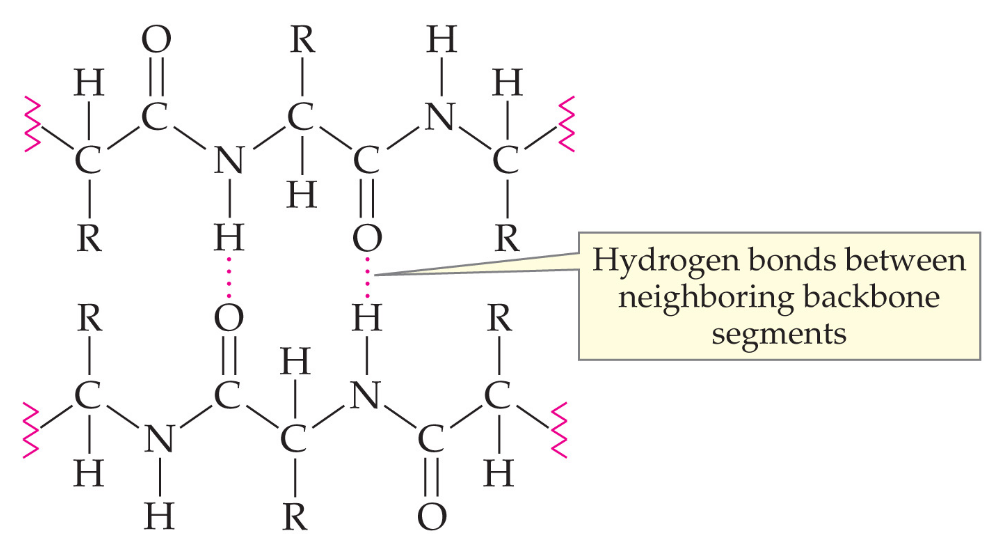
\includegraphics[width=.9\linewidth]{./images/protein-hydrogen-bond.png}
\end{center}

\newpage
\subsection{Tertiary structure of a protein (\(3^{\circ}\))}
\label{sec:orgea5d7ba}
The tertiary structure is the overall \textbf{three-dimensional shape} that results from the folding of a single protein chain. The tertiary structure mainly depends on \textbf{R group interactions} that are far apart along the entire backbone.
\subsubsection{Example 1}
\label{sec:org14c317e}
\begin{center}
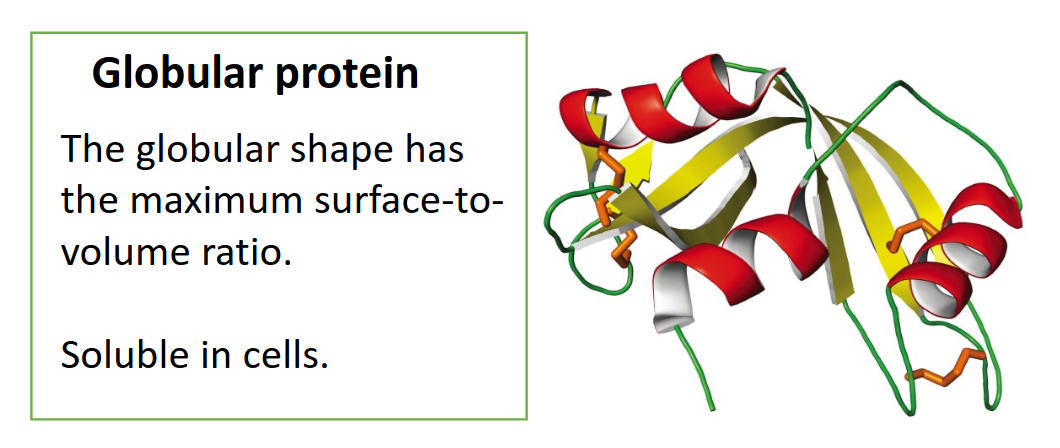
\includegraphics[width=.9\linewidth]{./images/globular-protein.png}
\end{center}
\subsubsection{Example 2}
\label{sec:orgde86c6e}
\begin{center}
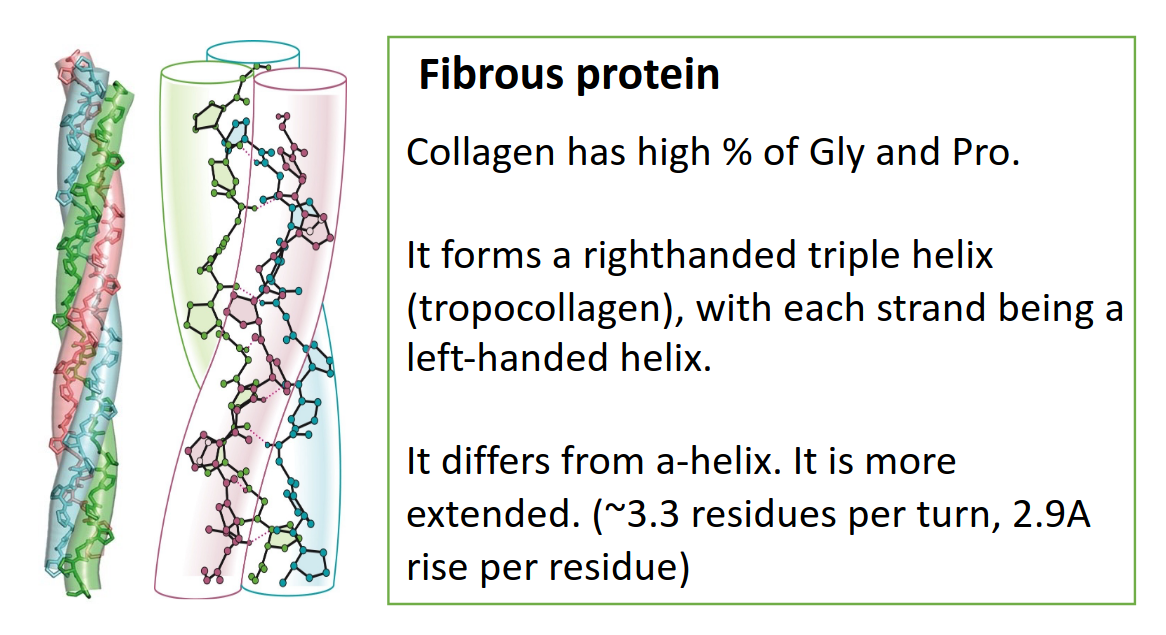
\includegraphics[width=.9\linewidth]{./images/fibrous-protein.png}
\end{center}

\newpage
\subsection{Quaternary structure of a protein (\(4^{\circ}\)) (tetramer)}
\label{sec:org4511a0e}
The quaternary structure of a protein consist of two or more interacting polypeptide chains, each of which is referred to as a subunit of the protein.
\subsubsection{Example}
\label{sec:orgb4c64fc}
\begin{center}
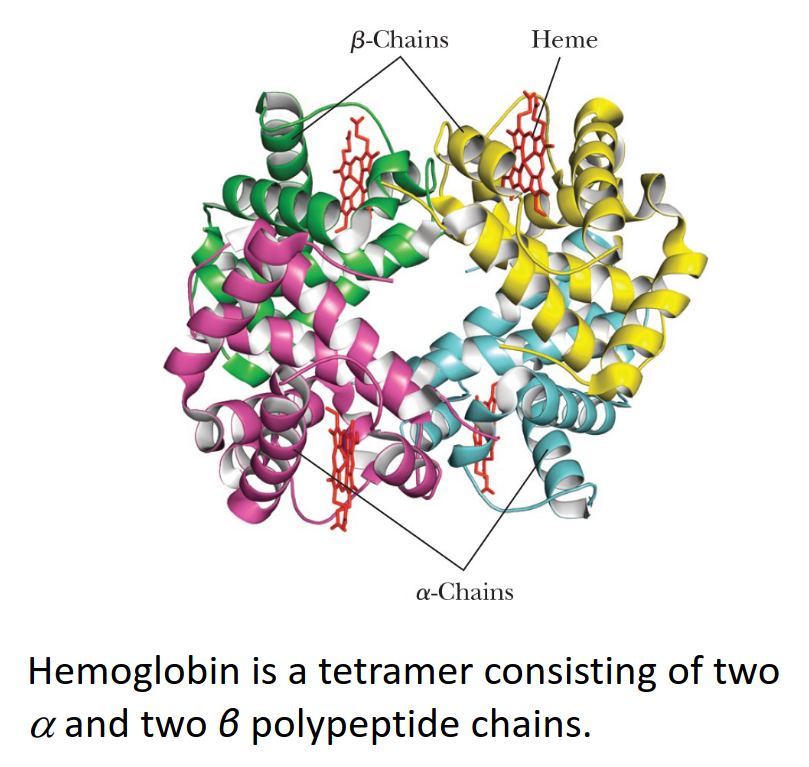
\includegraphics[width=.9\linewidth]{./images/hemoglobin.png}
\end{center}
\subsection{Subunit of a protein}
\label{sec:org044c5fe}
A subunit of a protein is a polypeptide chain that is inside a quaternary structure.
\subsection{Racemisation}
\label{sec:org06bf372}
Racemisation is a process in which optically active compounds consisting of a single enantiomer are converted into a racemic mixture, which is an equal mixture of enantiomers with no optical activity.
\subsection{Acid-labile}
\label{sec:orgc41f539}
Acid-labile just means that a compound is easily destroyed in an acidic environment.
\subsection{Acid hydrolysis}
\label{sec:org94fee92}
Acid hydrolysis is the method used to break peptide bonds, as it avoid racemisation and causes less destruction of certain amino acids such as \textbf{Ser}, \textbf{Thr}, \textbf{Arg}, and \textbf{Cys}.


The conditions are typically \(\qty{6}{\unit{M}}\) \(HCl\) at \(\qty{110}{\unit{\degreeCelsius}}\).


However, some amino acids are not compatible with acid hydrolysis and using acid hydrolysis will destroy the amino acid.
\begin{itemize}
\item \textbf{Trp} is not acid-compatible. UV light is used instead.
\item \textbf{Asn} and \textbf{Gln} are also acid-labile, and the side chain amino nitrogen is released as mmonium. \textbf{Asn} and \textbf{Gln} are converted to \textbf{Asp} and \textbf{Glu}.
\item The amount of \(NH_4^+\) released during acid hydrolysis gives an estimation of the total amount of \textbf{Asn} and \textbf{Gln}.
\end{itemize}
\subsection{Indole}
\label{sec:org11481a8}
The indole functional group is the one shown below. It is in the \(R\) group of tryptophan, \textbf{Tyr}.

\begin{center}
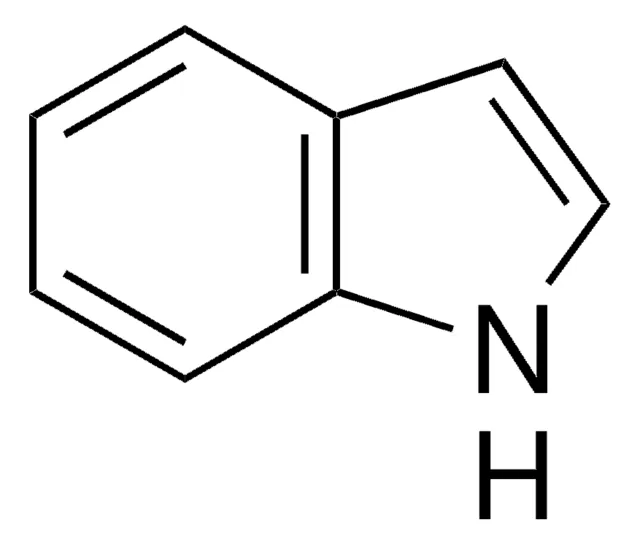
\includegraphics[scale=0.3]{./images/indole.png}
\end{center}

\newpage
\section{Structures and properties of amino acids}
\label{sec:org45ef25b}
\begin{itemize}
\item There are only 20 proteinogenic amino acids in nature.
\item The general structure of amino acids has an amino group (\(-NH_3^+\)) and a carboxylic acid (\(-COO^-\)), which are bonded to the alpha carbon (\(C_{\alpha}\)).
\item The side chain (\(-R\)) of amino acid is important for its properties
\item All amino acids are chiral except for glycine (\(G\)), where the side chain is a hydrogen atom (\(R = H\)).
\item Laevorotatory amino acids are predominant in nature.
\end{itemize}
\subsection{Spectroscopic properties of amino acids}
\label{sec:orgee93bab}
\begin{itemize}
\item Only tryptophan (\textbf{Trp}), tyrosine (\textbf{Tyr}) and Phenylalanine (\textbf{Phe}) absorbs UV light.
\item The absorbance at \(\qty{280}{\unit{nm}}\) is a good diagnostic device for amino acids.
\end{itemize}
\subsection{Acid-base properties of amino acids (amphoteric)}
\label{sec:org03e6263}
\begin{itemize}
\item The \(pK_a\) of the carboxylic acid group is about 2
\item The \(pK_a\) of the amino group is about 2
\item Therefore, at physiological pH, both the carboxylic acid group and the amino group will be ionised. This ionised form is called the \textbf{zwitterion}.
\item \textbf{Amino acids are typically written in their zwitterionic form.}
\end{itemize}
\section{Titration of an amino acid}
\label{sec:orgde3774c}
\begin{center}
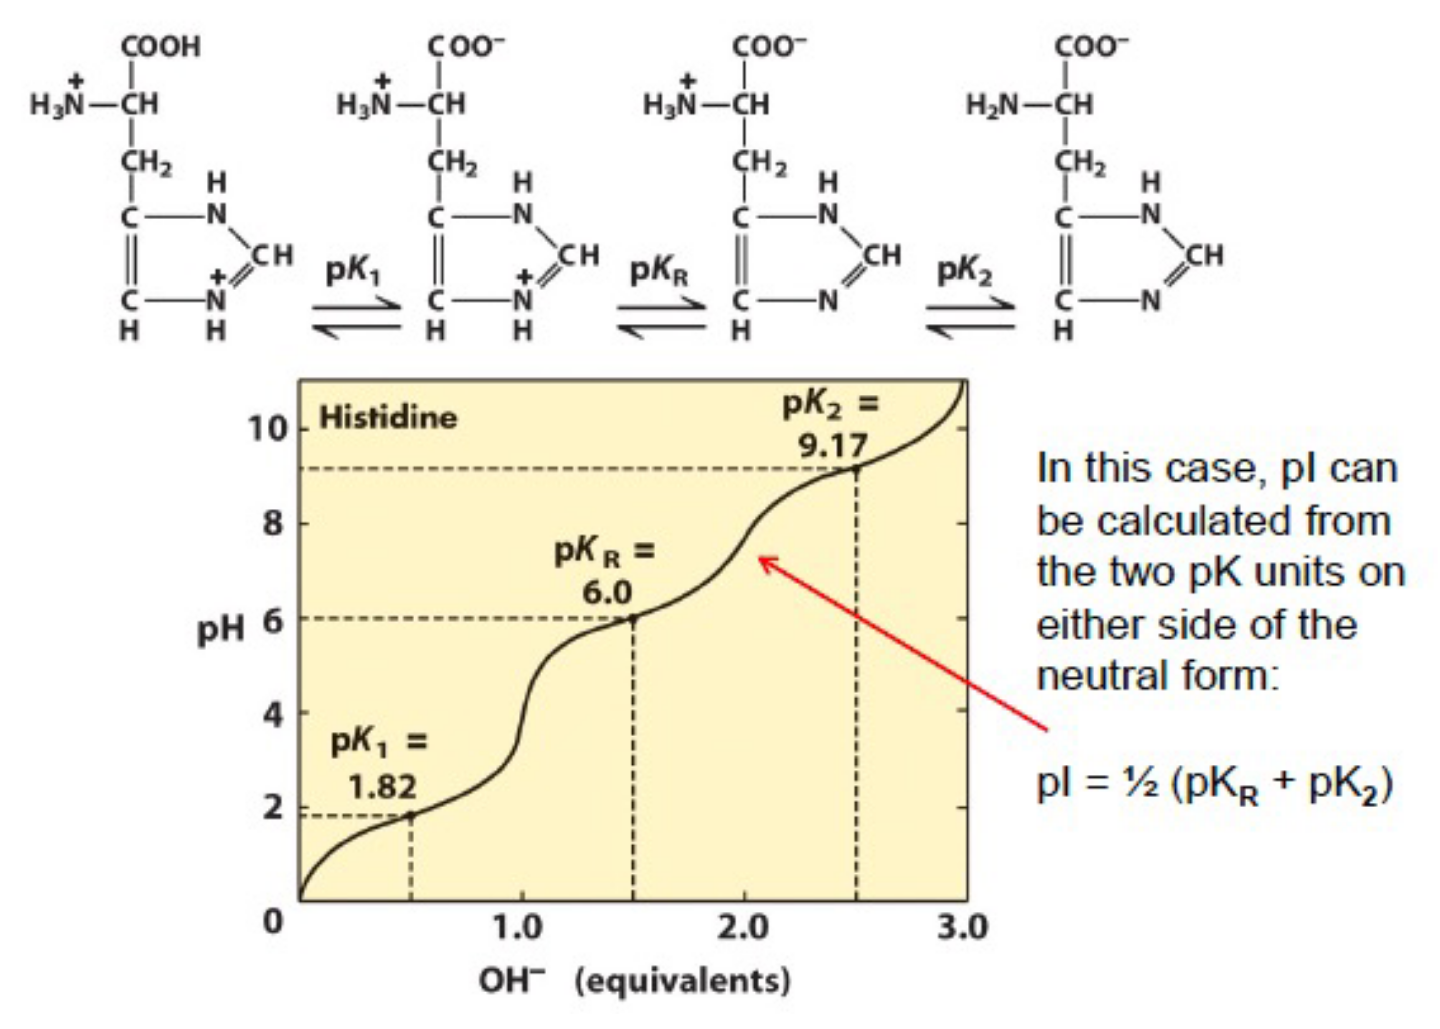
\includegraphics[width=.9\linewidth]{./images/titration-of-an-amino-acid.png}
\end{center}
\subsection{A useful formula}
\label{sec:orgedea562}
\[pH = pK + \log \left( \frac{[A^-]}{[HA]}\right)\]
\section{Disulfide bond formation by two cysteines}
\label{sec:org236847b}
\begin{center}
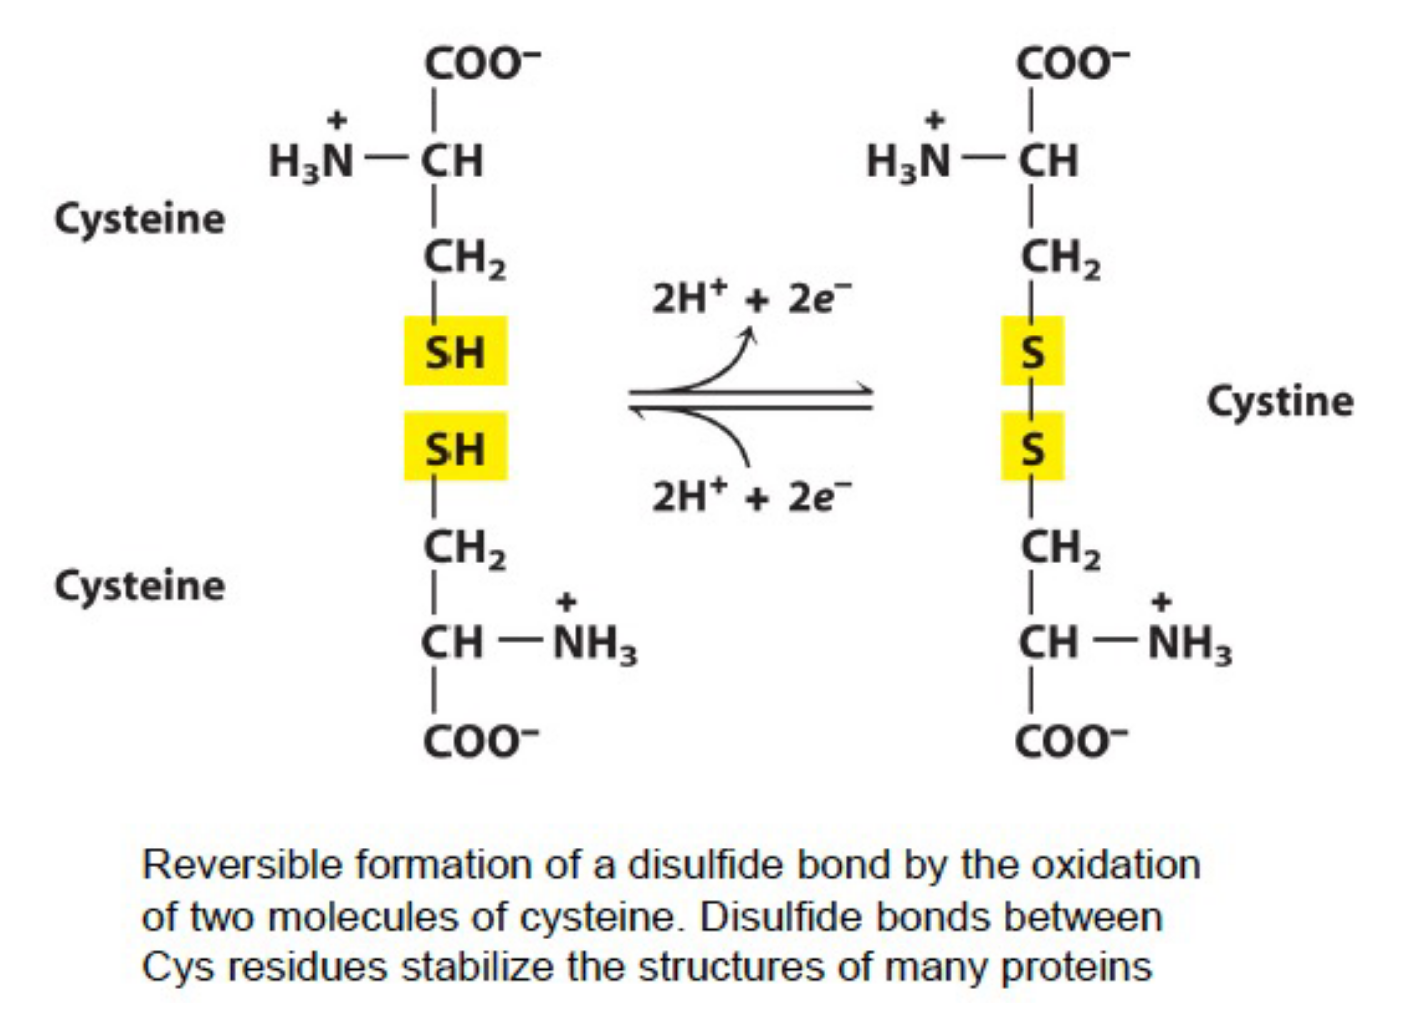
\includegraphics[width=.9\linewidth]{./images/cysteine-disulfide-bond-formation.png}
\end{center}
\section{Peptide bonds}
\label{sec:org9caa9bc}

\subsection{Peptide bond formation}
\label{sec:org1fce53e}
\begin{center}
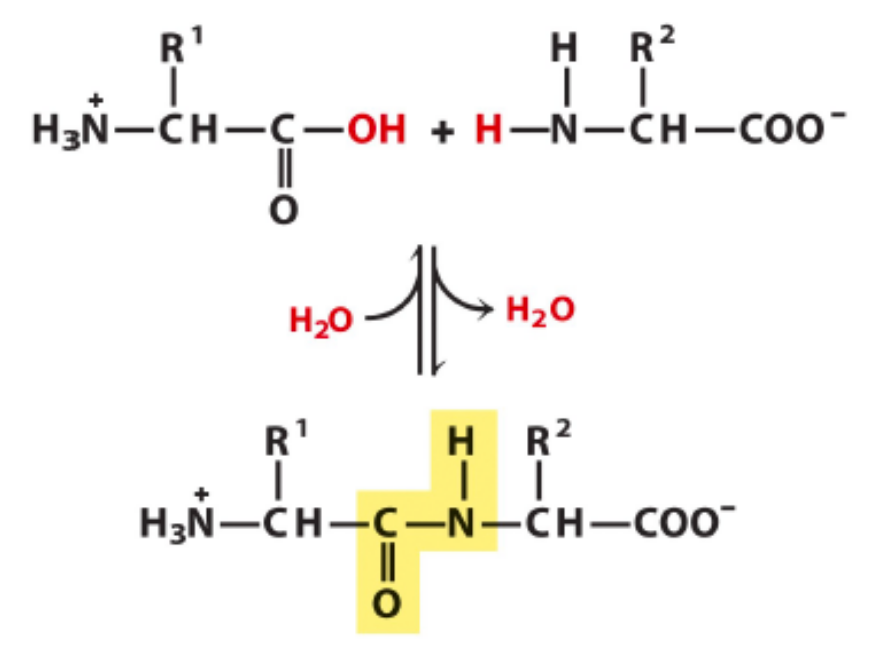
\includegraphics[width=.9\linewidth]{./images/peptide-bond-formation.png}
\end{center}
\subsection{Properties}
\label{sec:org99c7c22}
\begin{itemize}
\item Peptide bonds are \textbf{planar} with partial double bond character.
\item Due to the \textbf{partial double bond character}, the bond length is in between the typical single bond double bond, and the six atoms of the peptide bond groups are always in the \textbf{same plane}.
\item They are usually found in the \emph{trans} configuration as the \emph{cis} configuration has \textbf{steric hindrance}. The major exception is the peptide bonds in the sequence \(X-Pro\) where \(X\) is any other amino acid. Here, the \emph{cis} configuration is sometimes preferred, but the trans configuration is still favoured overall, with ratio of 4:1.
\item The amide \(N-H\) group is \textbf{partially positive}, and the carbonyl oxygen is partially negative, which results in a net dipole moment. Thus, the peptide bond is polar.
\end{itemize}
\section{Intermolecular interactions in protein structures}
\label{sec:org98b4b8f}
Non-covalent interactions stabilise the higher levels of the protein structure, like the secondary, tertiary and quaternary structures.

\begin{itemize}
\item \textbf{Hydrogen bonds} are formed whenever possible. These interactions are found on the peptide backbone and the polar residues.
\item \textbf{Hydrophobic interactions} drive protein folding, and they are usually found on the interior of the proteins and non-polar residues.
\item \textbf{Ionic interactions} usually occur on the protein surface. An example is the electrostatic interactions between opposite charges or repulsion between like charges.
\item \textbf{Van der waals} interactions are ubiquitous. An example is the instantaneous dipole-induced dipole interactions.
\end{itemize}
\section{Protein characteristics}
\label{sec:org37ff4d4}
\begin{itemize}
\item The unique characteristics of each protein is the \textbf{distinctive sequence of amino acid residues in its polypeptide chains}.
\item The \textbf{primary sequence} of proteins is encoded by the nucleotide sequence in DNA.
\item A polypeptide chain has two ends, the \textbf{N-terminus} and the \textbf{C-terminus}.
\end{itemize}
\section{Protein sequencing}
\label{sec:org3bb0ac5}

\begin{center}
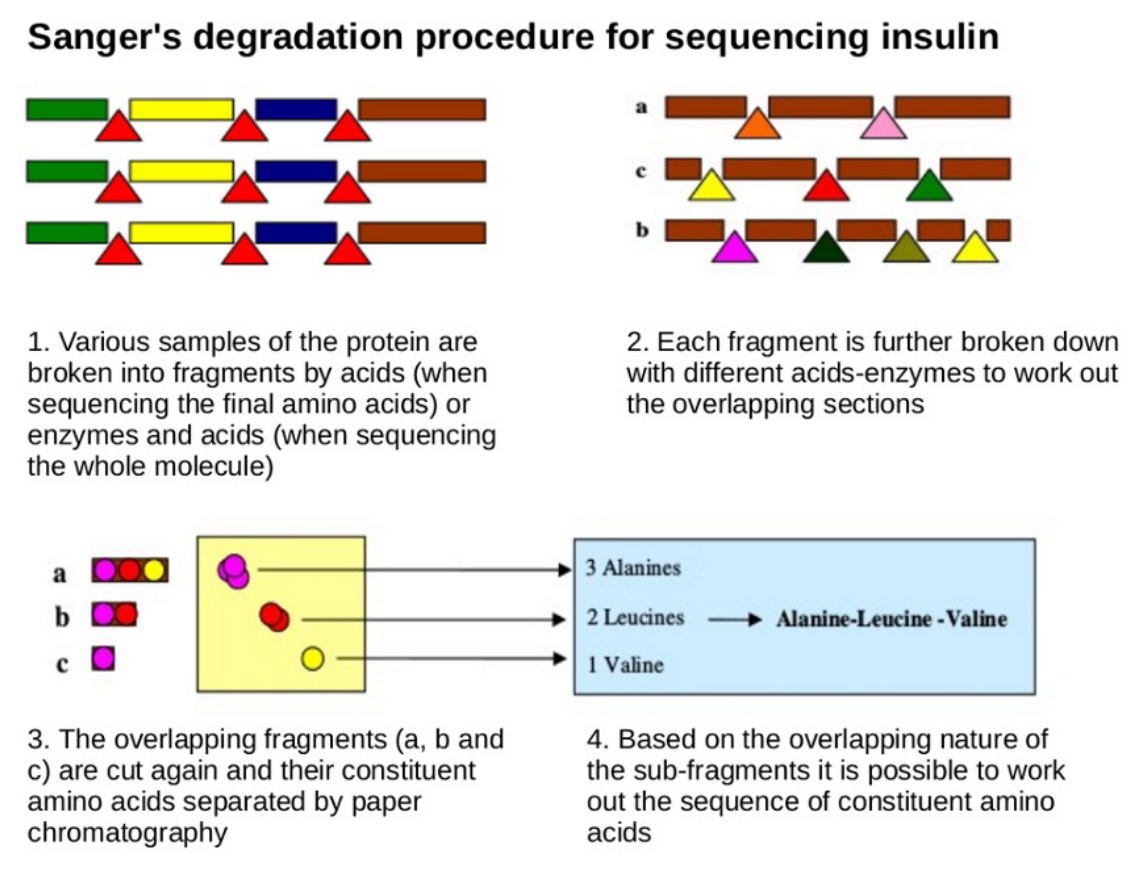
\includegraphics[width=.9\linewidth]{./images/protein-sequencing.png}
\end{center}
\subsection{Step 1}
\label{sec:orga1b098a}
\begin{itemize}
\item The interactions between protein subunits depend on weak forces, which are interactions that are not covalent, like instantaneous dipole-induced dipole interactions, permanent dipole-permanent dipole interactions and hydrogen bonding.
\item Hence, separation is achieved with:
\begin{itemize}
\item Extreme pH
\item \(\qty{8}{\unit{M}}\) urea
\item \(\qty{6}{\unit{M}}\) guanidine \(HCl\)
\item High salt concentration, usually ammonium sulfate
\end{itemize}
\end{itemize}

\newpage
\subsection{Step 2}
\label{sec:org66fdbe0}
Cleavage of disulfide bridges.
\subsubsection{Oxidation using performic acid}
\label{sec:orga04fded}
\begin{center}
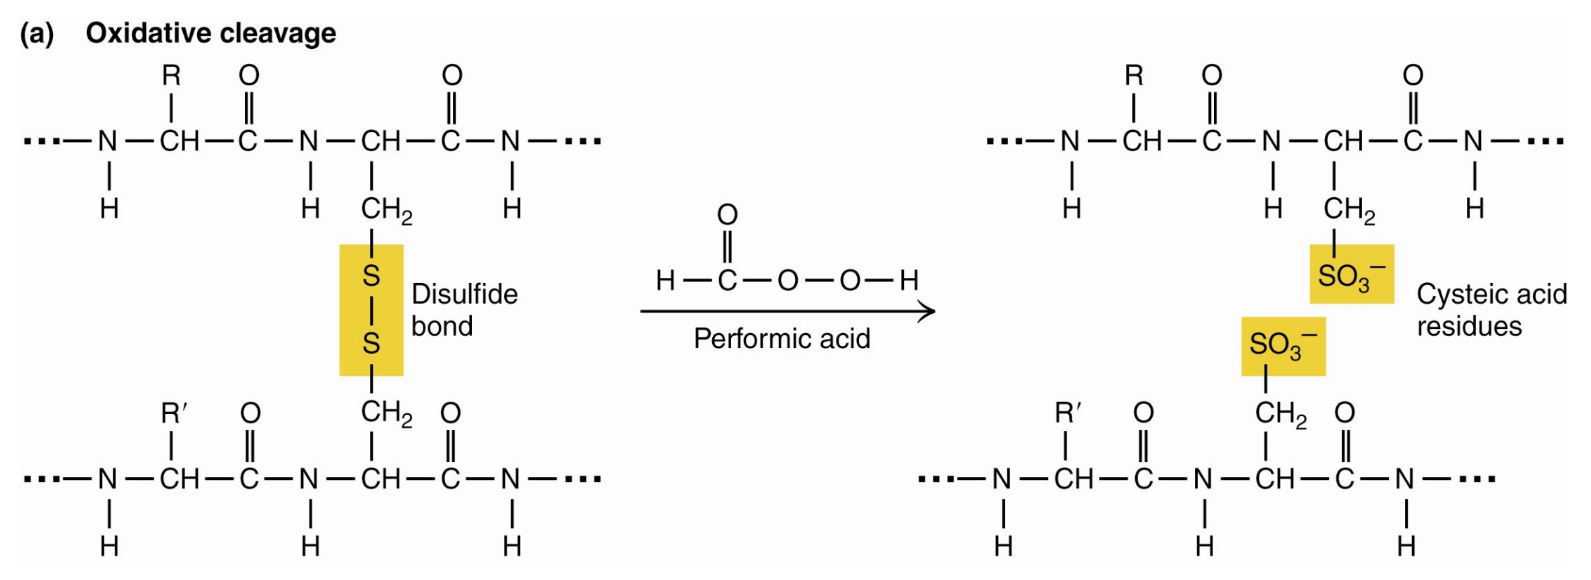
\includegraphics[width=.9\linewidth]{./images/oxidative-cleavage.png}
\end{center}
\subsubsection{Sulfhydryl reducing agnents}
\label{sec:org720c680}
\begin{itemize}
\item Examples include \textbf{mercaptoethanol}, \textbf{bME} or \textbf{dithiothreitol}, \textbf{DTT}.
\item To prevent recombination, alkylating agent like iodoacetate is used.
\end{itemize}
\begin{center}
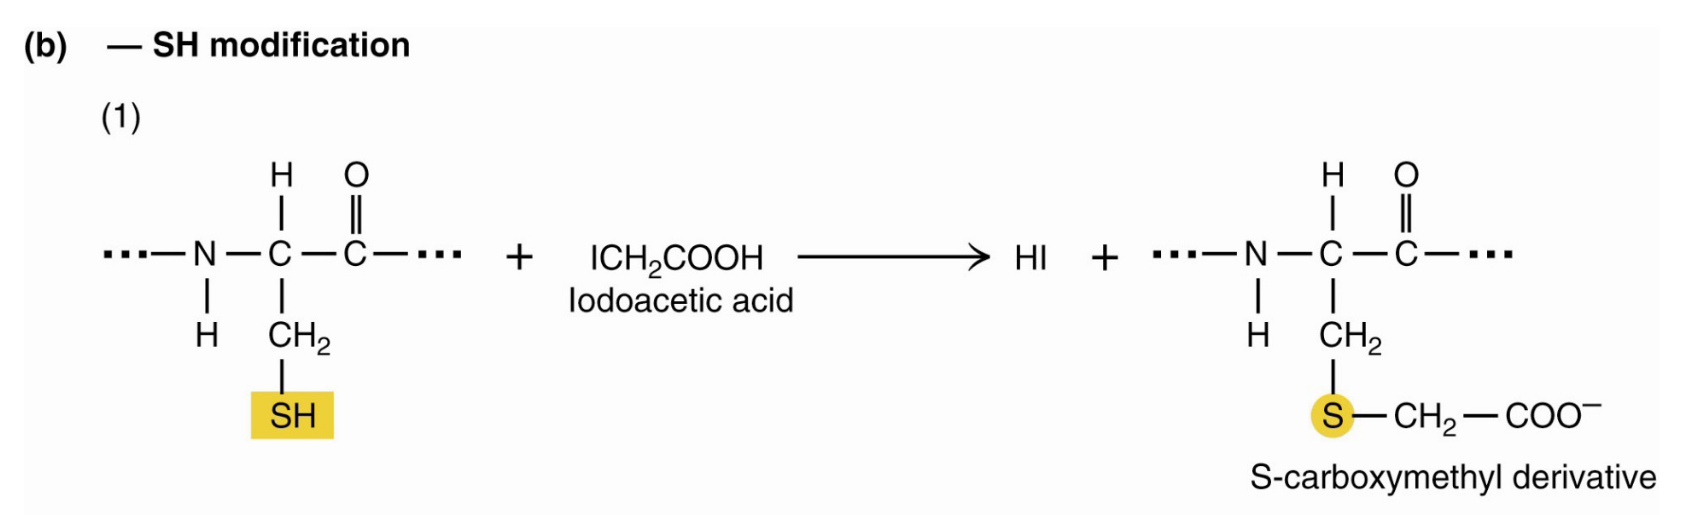
\includegraphics[width=.9\linewidth]{./images/reducing-sulfhydryl.png}
\end{center}

\newpage
\subsection{Step 3}
\label{sec:orgfc2c351}

\subsubsection{N-terminal analysis}
\label{sec:orgf2d1904}
\begin{itemize}
\item Edman's reagent (phenylisothiocyanate, PITC)
\item The reagent combines with the N-terminus of a protein, forming derivative phenylthiohydantoin derivative (PTH derivative)
\item Sequential Edman degradation is also possible
\end{itemize}
\begin{center}
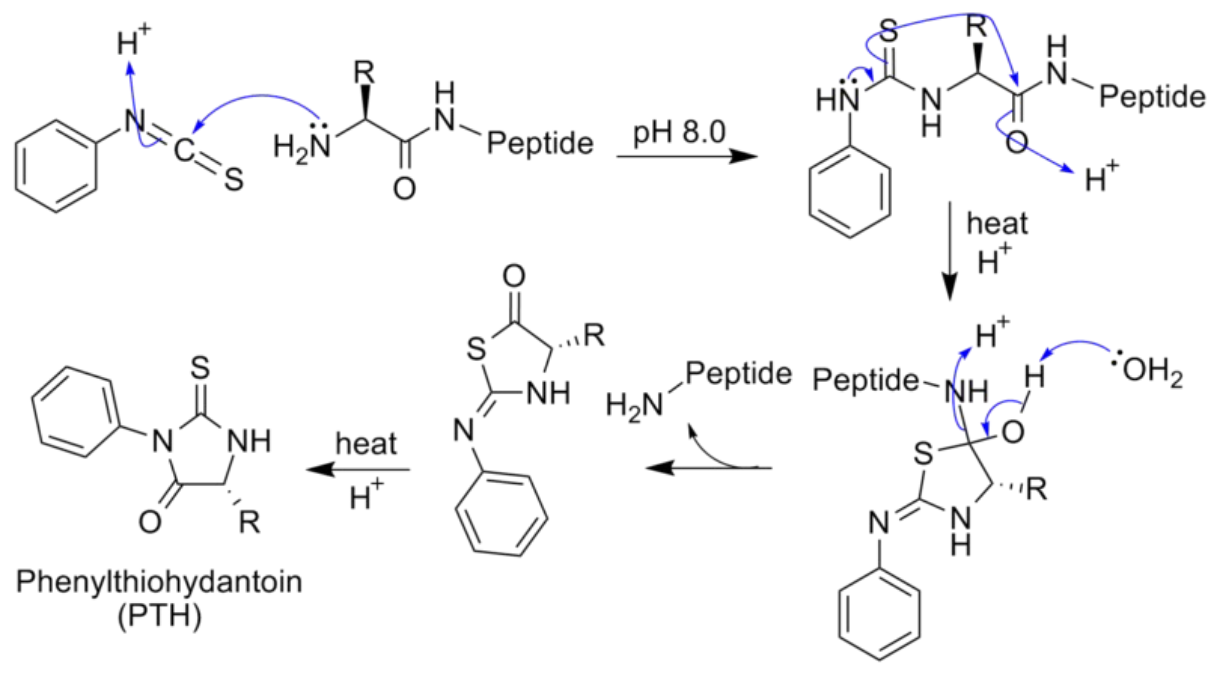
\includegraphics[width=.9\linewidth]{./images/edman-degradation.png}
\end{center}
\subsubsection{C-terminal analysis}
\label{sec:org9f6e301}
\begin{itemize}
\item Enzymatic analysis (carboxypeptidase)
\item \textbf{Carboxypeptidase A} cleaves the N-side of any residue at the C-terminal position except \textbf{Pro}, \textbf{Arg}, \textbf{Lys}, \textbf{Glu}, \textbf{Asp}.
\item \textbf{Carboxypeptidase B} (hog pancreas) only works on the N-side of \textbf{Arg} and \textbf{Lys} at the C-terminus.
\item \textbf{Carboxypeptidase Y} (yeast) works with any residue.
\end{itemize}

\newpage
\subsubsection{Fragmentation of polypeptide chains}
\label{sec:org2222963}
\begin{enumerate}
\item Enzymatic fragmentation
\begin{itemize}
\item This is done using \textbf{trypsin}, \textbf{chymotrypsin}, \textbf{clostripain}, \textbf{staphylococcal protease}.
\item Trypsin cleaves on the C-side of Lys and Arg.
\item Chymotrypsin cleaves on the C-side of Phe, Tyr and Trp.
\item Clostripain only cleaves on the C-side of Arg.
\item Staphylococcal protease cleaves on the C-side of Asp and Glu.
\end{itemize}

\item Chemical fragmentation
\begin{itemize}
\item \textbf{Cyanogen bromide (CNBr)} acts on the C-side of methionine residues.
\item It is useful as proteins usually only have a few Met residues.
\item The use of cyanogen bromide is indicated by a homoserine lactone at the C-terminal of the peptide. Homoserine lactone refers to the ring structure in the product in the picture below. The presence of that structure means that methionine is present and cyanogen bromide was used.
\end{itemize}
\end{enumerate}
\begin{center}
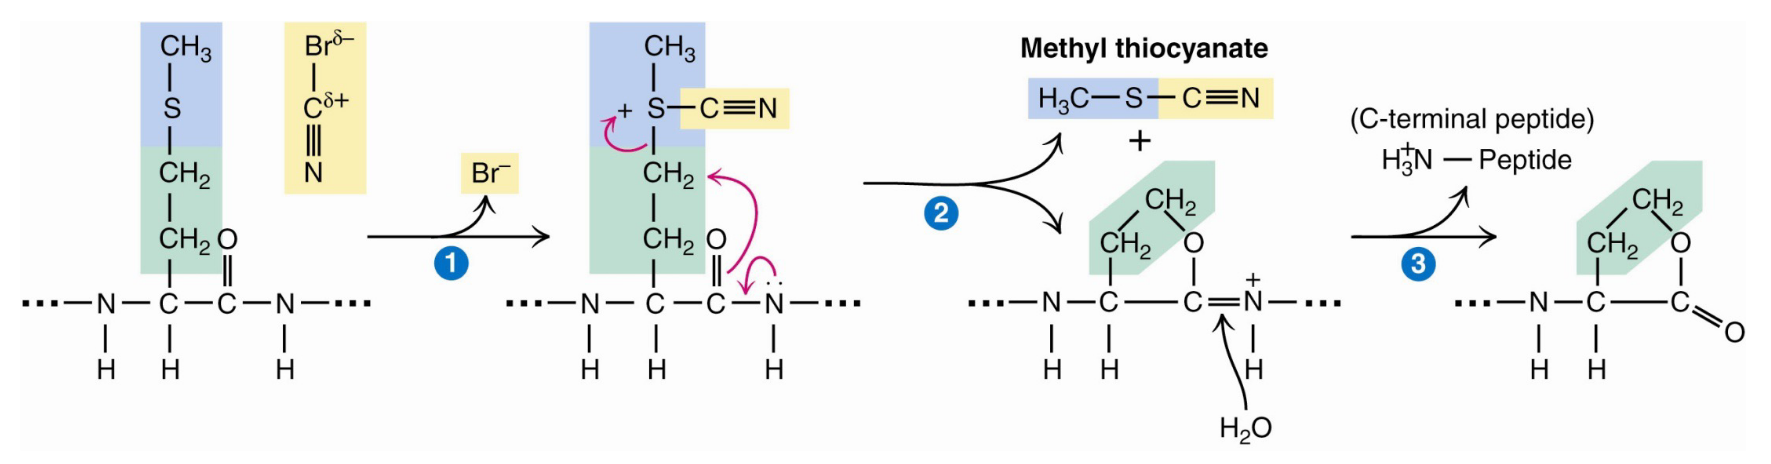
\includegraphics[width=.9\linewidth]{./images/cyanogen-bromide-fragmentation.png}
\end{center}
\end{document}
